\label{ch:LitReview}
\textit{This chapter covers the system dynamics and the model used for simulation and control. It then moves on to a more thorough review of the control techniques available for the problem solution.}

\section{System Identification and Modeling}
The system could be described as repeatedly going through two sequential phases, the setup phase and the steady state phase, which together form what will henceforth be called a transmission round. The setup phase is when the transmission structure and hierarchy among the network's living nodes occurs. The steady state phase is when transmission is executed all the while adjustments are made to the sink position and the PR of the nodes. 

\subsection{Clustering}
There have been several network routing protocols proposed in the context of wireless sensor networks. Two of these are minimum-transmission-energy (MTE) and static clustering, but none of these economizes network energy consumption and increases node longevity as well as LEACH. LEACH has shown to increase the network lifetime by as much as eight times compared to the aforementioned alternatives. \cite{heinzelman2000energy} .\newline

\noindent LEACH works by each node individually deciding whether or not to become a cluster head for each sequential round during the setup phase. The decision is made by producing a threshold value $T(n) \in [0:1]$, see Equation \ref{leacheq}, and comparing this value to a random number in the same value range. If the number is less than threshold $T(n)$, the node becomes a cluster-head for the current round. The threshold is set as
\begin{equation}
\label{leacheq}
    T_{LEACH}(n) = \begin{cases} \frac{P}{1-P(n\,mod\frac{1}{P})}, & \mbox{if } i \in G\\ 0, & \mbox{otherwise} \end{cases}
\end{equation}
where $P$ is the desired percentage, set a priori, of cluster heads (e.g. $P = 0.05$), $n$ is the current round. $G$ is the set of nodes that have not yet been cluster-heads in the current \textit{cycle}, where a cycle is defined as $\frac{1}{P}$ rounds. As can be seen in Figure \ref{fig:LEACHplot}, each node will be a cluster-head at some point within a cycle \cite{heinzelman2000energy}.\newline

\begin{figure}
    \centering
    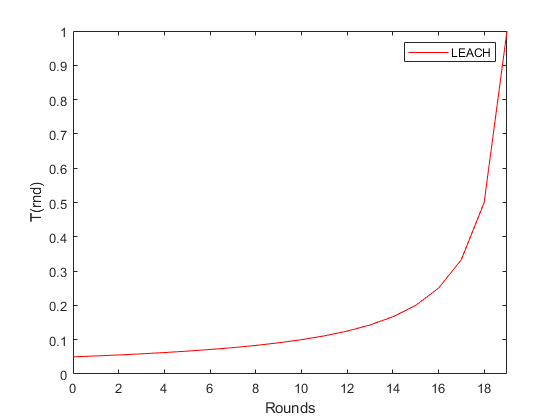
\includegraphics[scale=0.9]{Images/LEACHplot.png}
    \caption{Value of T(n) over one cycle with $P=0.05$}
    \label{fig:LEACHplot}
\end{figure}

\noindent After cluster heads have been chosen for a round it works like a regular LEACH protocol. All other nodes simply connect to whichever cluster head is closest, which is the cluster head that provides the strongest signal. This can be done with a CSMA MAC protocol that works by letting all nodes listen if there is some signal already broadcasting. If there is, the node waits a randomly generated amount of time until listening and trying again; if there is no signal, then it broadcasts and tries to connect to the nearest cluster head. The cluster head then assigns a TDMA schedule to each of it sub-nodes so that each node knows exactly which time window it is supposed to broadcast on.
Finally, as soon as clusters have been formed the cluster heads starts relaying data from it's connected nodes to the sink. When all the data has been received by the cluster head, it performs signal processing functions to compress the data into a single signal. For example, if the data are audio or seismic signals, the cluster-head node can beamform the individual signals to generate a composite signal \cite{heinzelman2000energy}.

\subsection{Sink Movement and Data Flow}
\label{subsec:sinkDataFlow}
% MAKE SURE THE MIXED INTEGER THINGY IS EXPLAINED IN MODEL DESCR
The equations governing the energy and data aggregation dynamics of each node in the system are derived from \cite{heinzelman2000energy} and are expressed as
\begin{flalign}
    E_{Tx}(b_{tx},d) &= E_{elec}b_{tx}+ E_{amp}b_{tx}d^{2} \\
    E_{Rx}(b_{rx}) &= i(E_{elec}+E_{DA})b_{rx} \\
    \Psi &= E_{Tx} + E_{Rx} - E_{gen}
\end{flalign}
where $b$ is amount of bits either transmitted ($tx$) or received ($rx$), $d$ is the distance between transmitter and receiver and $i$ is the number of nodes connected. $E_{Tz}$ and $E_{Rz}$ represent energy consumed for transmission and receiving respectively, $E_{gen}$ represent energy generated, and $\Psi$ represents the sum of these. $E_{elec}$, $E_{amp}$ and $E_{DA}$ are constants related to power circuit consumption.
Here, a CH performs both transmission and reception while non CHs only do transmitting. Each node is also able to stochastically generate a relatively small amount of energy during each time step. \newline

\section{Control Strategies}
\label{sec:ctrlstrategies}
\noindent In order to achieve a model based controller for a multi-variable system with two contradicting economic goals, multiple optimal control methods were considered. To determine the feasibility of the methods, a study of their respective advantages and limitations was conducted.\newline

\noindent Three popular model based optimal control methods were considered. These were MPC, dynamic programming (DP) and linear quadratic regulation (LQR). All these methods work by calculating an optimal sequence of control steps into the future, where the optimal sequence is defined by an objective function. \cite{grune2019dynamic}.\newline

\noindent DP calculates a global optimum via backward calculation. This means that each optimization problem starting from the horizon requires the prior optimization problems leading up to it to be defined \cite{grune2019dynamic}. Due to the stochastic dynamics and nonlinearities of the system, this would not be computationally feasible for controlling the entire system in practice. \newline

\noindent On the other hand, an online optimization method such as MPC or receding horizon LQR need only to act upon an approximation of the future states, consequently generating a sub-optimal but feasible solution. However, the receding horizon LQR is meant to be applied on linearly constrained models where the cost function is quadratic.\newline

\noindent Since the system at hand is nonlinear and subject to hard constraints such that
\begin{itemize}
    \item each node can only be controlled if it has attained CH role
    \item there is a limit to the amount of packets a node can send during a round
    \item there is a limit to the step length of the sink
\end{itemize}
the receding horizon LQR is not feasible. In contrast to this, constrained and nonlinear optimal control is what MPC famously excels at \cite{MPCbook}.\newline

\noindent A counterpart to model based control is the data driven approaches, such as simulated annealing, artificial neural networks (ANN) and RL. The simulated annealing method finds a global optimum after iterating over a period of time for a system that does not change. Since it is a possibility that the proposed control problem runs for an indefinite amount of time and has an ever changing optimum it is not feasible to use the simulated annealing algorithm. In this case, the use of an ANN is not feasible due to the reason that the desired movement of the sink is unknown. It is therefore not possible to calculate the error between the reference value and output value which is needed to update the weights of the ANN. \newline

\noindent An RL algorithm such as Q-learning and SARSA are model free, i.e. the model of the system is not needed for controlling the system. Instead, the system chooses actions and receives a user defined reward which is based on the chosen action. Since high PR and low EC is desired, there is an easy method to reflect the desired behaviour onto the reward given to the system. Thereby, the most feasible data driven controller to employ on the proposed system is RL. 

\section{MPC}
\label{nonlinMPC}
The nonlinear MPC (NMPC) control algorithm calculates its optimal control input sequence through numerically optimizing for a minimum or maximum value of an objective function $J^{*}=min/max\:C(x,u)$ \cite{MPCdimitry}. This is done in a receding horizon fashion, meaning that it only implements the first control action and then repeats the planning at every new sampling instant \cite{MPCbook}. By defining $J^{*}$ as a function dependent on an accurate model of the dynamics of the system as well as desired constraints on the solution, the system can be controlled towards a desired state with an optimal trajectory. In this case, optimality could be defined with regards to costs such as time or energy consumption. Another benefit of MPC is its capacity of handling multi-input multi-output systems that may have interactions between their inputs and outputs \cite{MatlabMPC}. However, one ought to take into consideration that with multiple variables comes an ever increasing computational load on the controller as the time complexity of the algorithm is $\mathcal{O}((nN)^{3})$ with $n$ and $N_c$ denoting the number of controlled inputs and the control horizon, respectively \cite{li2011application}.\newline

\noindent For a mathematical formulation of the NMPC problem, the stabilization problem for a systems described by a nonlinear set of
equations can be considered as
\begin{equation}
\label{ss-dynamic}
    x(k+1) = f(k, x(k), u(k), d(k)),\; x(0) = x_{0}
\end{equation}
Subject to state and input constraints
\begin{align}
     u(k) \in \mathcal{U}, \forall k\geq0 \; x(k) \in \mathcal{X}, \forall x \geq 0
\end{align}
Where the set of feasible input values is denoted by $\mathcal{U}$ and the set of feasible states is denoted by $\mathcal{X}$. For solving the optimization problem, it is assumed that $\mathcal{X}$ and $\mathcal{U}$ satisfy the following assumptions \cite{findeisen2002introduction}:
\begin{itemize}
    \item $\mathcal{U}$ is compact, $\mathcal{X}$ is connected and $(0,0)\in\mathcal{X}\times \mathcal{U}$
    \item The vector field $f$ is continuous and satisfies $f(0,0) = 0$
    \item The system \ref{ss-dynamic} has an unique continuous solution for any initial condition in the region of interest and any piecewise continuous and right continuous input function
\end{itemize}

\noindent For $J$, the standard quadratic form is the simplest and most often used one and can be described as follows
\begin{equation}
    Minimize\:J(x(k),u(k)),\: J=\sum_{k=0}^{K-1} x^{T}Qx + u^{T}Ru
\end{equation}
where Q and R denote positive definite, symmetric weighting matrices, $K$ is the control horizon length in discrete time steps, $x(k)$ is the system state vector at discrete time step $k$, $u(k)$ is the control input vector at discrete time step $k$.\newline

\noindent $J$ would also be subject to constraints for $k\in[0,\hdots,T-1]$ with the following forms
\begin{align}
    \mathcal{A}x(k) &+\mathcal{B}u(k)\leq \phi, \phi(k)  \label{leqeq}\\
    \mathcal{A}_{eq}x(k) &+\mathcal{B}_{eq}u(k) = \phi_{eq}, \phi_{eq}(k) \label{eqeq}
\end{align}
\noindent Here, $\phi$ and $\phi_{eq}$ are stated as either constants or dynamic vectors.

\subsection{Mixed-Integer Nonlinear Programming}
Mixed-Integer Nonlinear Programming (MINLP) problems are defined as those where some or all of the decision variables are only allowed to be integers. This is typically required in a range of real world applications in allocation and planning problems where the discrete variables represent quantities and require integer values for the solution. \newline

\noindent A common method of solving for integer representations of the decision variables is by using the "Branch and Bound" method. It works by initially finding the optimal solution to a relaxation of the problem without the integer constraints, via standard linear or nonlinear optimization methods. Thus, it results in a greater chance that the problem satisfies the previously stated assumptions. The method then branches out from the non-integer solution by creating several more tightly constrained sub-problems around the optimal point to find a solution that satisfies all the integer constraints \cite{frontlineSolversMIP}.\newline





\section{RL Theory}
 In a RL algorithm, e.g. Q-learning and SARSA, the so called agent learns without labeled data by executing actions $a$ from a pre-detemined action set $\mathcal{A}$ such that $a \: \in \: \mathcal{A}$. After performing the action, the agent evaluates the outcome of the action based on rewards, $R_t \: \in \: \mathcal{R} \: \subset \mathbb{R}$, from the environment where $\mathcal{R}$ is the set of rewards. The objective is to maximize the reward that the agent gains after each episode, i.e. after every iteration of the entire algorithm. The agent starts from an arbitrary initial state and receives a new state from the environment after performing an action. If the action is desired the agent will also receive a positive reward and vice versa, see Figure~\ref{fig:RLoverview}. The maximum reward that the agent can receive is determined by solving the Bellman equation which is the sum of the reward that the system obtains immediately by taking the action and the amount of future rewards that the agent can receive at the new state \cite{sutton2018reinforcement}. Further, in order to enable a trade off between exploitation of maximizing reward and exploration of the environment for the agent, a probability of $\epsilon$ is introduced for taking a random action. $\epsilon$ is the exploration rate and the agent will take a random action with a probability of $\epsilon$ \& will take the action that yields the highest reward with a probability of $1-\epsilon$. This method to explore the environment is needed due to that there could be sub-optimal states and is called $\epsilon$-greedy exploration. 

\begin{figure}[H]
  \centering
  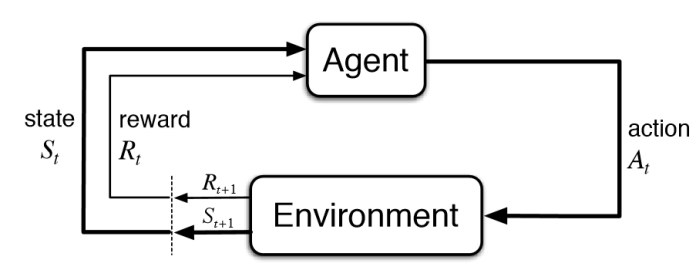
\includegraphics[width=0.9\textwidth]{Images/RLoverview.jpg}
  \caption{Overview of reinforcement learning algorithm \cite{sutton2018reinforcement} } 
  \label{fig:RLoverview} 
\end{figure}

\subsection{Q-learning}
\noindent  Q-learning is an RL algorithm that is model free. The algorithm finds the best action for a state by solving the Bellman equation stated in Equation \ref{eq:bellman}.

\begin{equation}
\label{eq:bellman}
    Q(s,a) = r + \gamma \max_{a'} Q(s',a')
\end{equation}

\noindent Here $Q(s,a)$ is called the quality-value (Q-value) and is the action-state value for a given state and action, $r$ is the immediate reward of an action, $\gamma$ is the discount factor for future states and $\max_{a'} Q(s',a')$ is the maximum future Q-value that can be obtained with a new action $a'$ given a new state $s'$. Thereby, Equation \ref{eq:bellman} states the immediate reward of an action and the maximum reward that the agent can receive when the agent has entered a specific state. The idea behind Q-learning is to iteratively update the Q-values, i.e. $Q(s,a)$, for every state-action pair such that it converges towards the optimal Q-value, $Q^*(s,a)$. At each iteration step, the Q-value is updated as in Equation \ref{eq:QValueIter} \cite{sutton2018reinforcement}.

\begin{equation}
\label{eq:QValueIter}
    Q_{t+1}(s_t,a_t)=Q_{t}(s_t,a_t)+\alpha(r_{t+1} + \gamma \max_{a} Q_t(s_{t+1},a)-Q_{t}(s_t,a_t))
\end{equation}

\noindent In this case $Q_{t+1}(s_t,a_t)$ is the updated Q-value from the previous Q-value $Q_{t}(s_t,a_t)$ and $\alpha$ is the learning rate which determines how much the difference between the new Q-value and the old Q-value affects each iteration step. The agent updates the Q-value with Equation \ref{eq:QValueIter} by randomly choosing actions from the action set with an $\epsilon$ probability and by choosing the action that the agent predicts would yield the most reward with a probability of $1-\epsilon$.

\subsection{Deep Q-Network}

The main disadvantage with the Q-learning algorithm is that the agent needs to step through every state-action pair multiple times to get a reasonable Q-value for all state-action pairs. Therefore, it becomes rapidly infeasible to solve the problem in a timely manner when the amount of states and actions are increased due to the curse of dimensionality. A RL algorithm that is more suitable for a large number of states and actions is deep Q-networks (DQN) which is an extension of the Q-learning algorithm.\newline

\noindent Instead of naively updating the Q-value when the agent reaches a state-action pair, the DQN algorithm approximates the Q-value of the state-action pair with a neural network (NN). The role of the NN is to map the states of the environment with the action that is optimal for the agent to take. In other words the NN determines which action is the most optimum, i.e. has the highest Q-value, for a specific state \cite{silver2013DQN}. \newline 
\newline
\noindent To train the agent, there is a need for expressing the difference between the prediction of the NN and the actual target value mathematically. The agent's loss is a value that is a quantitative measure of how good a prediction is. By using an optimizer the loss as a mean absolute error (MAE), and thereby also the NN's prediction error, is minimized. Equation \ref{eq:mse} depicts the MAE where $n$ is the amount of data points to be optimized for.   

\begin{equation}
    \label{eq:mse}
    MAE = \frac{1}{n}\sum^{n}_{t=1}(loss) 
\end{equation}

\begin{equation*}
         where \hspace{0.25cm} loss =  |\underbrace{r + \gamma \max_{a_{t+1}} Q_t(s, a_{t+1})}_{Target} - \overbrace{Q_{t}(s_t,a_t)}^{Prediction}|
\end{equation*}

\noindent The optimizer does all of the work of minimizing the loss by tuning the weights of the NN based on the absolute error between the target and the NN output. This leads to a converging Q-value and a decreasing loss. After the best action was performed and the weights of the NN are updated the DQN algorithm follows the Q-learning algorithm until the next occasion an action is to be selected. 

\subsection{Neural Network}

A neural network is a field within machine learning. The main usage of a NN is to find a pattern between a given input and an output by mimicking the biological structure of a brain with its dendrites and synapses \cite{SiddiqueNH2013Ciso}. In a NN the basic building block is called a neuron and by connecting a number of neurons a NN is formed. As seen in Figure \ref{fig:NNoverview} the neurons are ordered in layers in which the first layer is the input layer and the last layer is the output layer. Each neuron in the input layer corresponds to one variable, i.e. one input, and between the input layer \& the output layer there are an arbitrary amount of hidden layers. Additionally every edge, i.e. every connection between two neurons, has a weight associated with it. It is these weights that determine the output of a neuron based on a given input. \newline       

\begin{figure}[h]
    \centering
    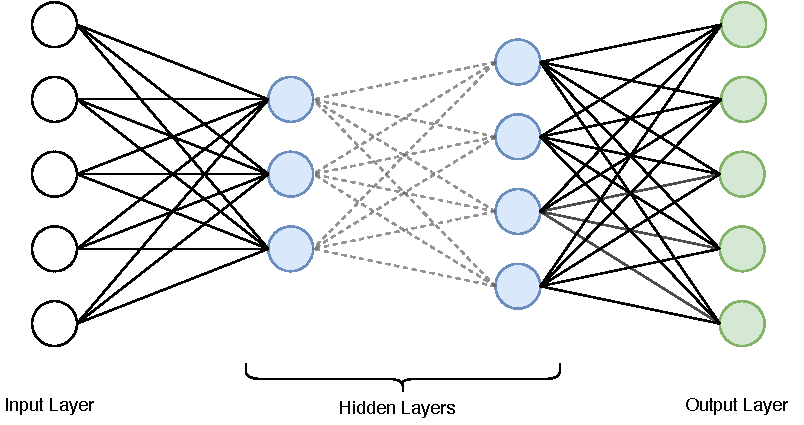
\includegraphics[scale=1]{Images/NNoverview.pdf}
    \caption{Overview sketch of a NN}
    \label{fig:NNoverview}
\end{figure}

%\vfill \break
\noindent The learning process starts when data is provided to the input layer. By using the edge's weights the NN calculates the output value of all the neurons in the output layer. The NN then uses the difference between the calculated output \& the expected output to update the weights via an optimization algorithm in order to make better predictions in the future. This process of improving the weights is called error backpropagation. The role of the optimization algorithm is to minimize the loss of the NNs predictions by updating the edge's weights based on gradient descent \cite{SiddiqueNH2013Ciso}.  

\subsubsection{Remember, Memory and Replay}
\noindent One major issue with the DQN algorithm is that the NN has a tendency of forgetting what was learned previously when it overwrites them with new experiences. Therefore, a remember function needs to be used to append the previous observations and experiences onto an array named memory. After every action, the agent replays a number of randomly chosen experiences from its memory and the weights of the NN are once again fitted based on these experiences \cite{lin1992self}. 


\section{Software Tools}
\label{sec:softwaretools}
Some parts required for the controllers' basic structure were already available through libraries. This section presents options considered for the tasks.


\subsection{Optimization Tool}
A couple of different libraries were considered for simplifying and streamlining the process of solving the optimization problems related to the optimal control approach. \newline
\newline
\noindent \textbf{CasADi} is an open-source tool for nonlinear optimization and algorithmic differentiation.
It facilitates rapid — yet efficient — implementation of different methods for numerical optimal control, both in an offline context and for nonlinear model predictive control (NMPC) \cite{Andersson2018}. The tool is compatible with both Matlab and Python.\newline

\noindent \textbf{GEKKO} is a Python package for machine learning and optimization of mixed-integer and differential algebraic equations. It is coupled with large-scale solvers for linear, quadratic, nonlinear, and mixed integer programming (LP, QP, NLP, MILP, MINLP). Modes of operation include parameter regression, data reconciliation, real-time optimization, dynamic simulation, and nonlinear predictive control \cite{beal2018gekko}.\newline

\noindent Both libraries offer sufficient means for continuously solving non-linear optimization problems. However, in the opinion of the authors at that moment, GEKKO offered far better support and guidance in the form of an active user forum and example material.

\subsection{Machine Learning Tool}
Two of the most established machine learning libraries that are compatible with Python are pyTorch and TensorFlow. Below follows a short description of both machine learning libraries. \newline
\newline
\noindent \textbf{PyTorch} is a deep learning framework that is based on Tourch \cite{paszke2017automatic}. It has a simple interface, is easily extendable and integrates into Python smoothly. The computational graph in pyTorch is updated dynamically which means that the graph is updated at runtime and hence it is easier to debug. \newline 
\newline
\noindent \textbf{TensorFlow} is an open-source library that can be used to build and train machine learning models \cite{tensorflow2015-whitepaper}. When using this library it is possible to add an abstraction level by building the model on an application programming interface (API) called Keras \cite{chollet2015keras}. Further, TensorFlow provides a vast range of material which aids the learning process.\newline   
\newline 
\noindent PyTorch and TensorFlow are both capable libraries and could solve the RL problem. Nevertheless, the Keras API which runs on top of TensorFlow had a larger community, better guidance and documentation. For setting up the WSN environment in a reinforcement learning context, the gym library from OpenAI provides a straightforward procedure to model the reward \cite{open160601540}.


%For controlling the mobile sink with RL, it was decided to run Keras on top of TensorFlow.